\section{问题三：基于阈值首达判据的烘干时长模型}
\label{sec:p3}

\subsection{相对问题二的增量}

问题三与问题二求解的是同一个初边值问题：附录 3 物性全程统一、
半径固定为 $R_0$、烘房条件按第~\ref{sec:model}~节的约定延拓。
唯一新增的内容是终止判据，即由“给定时刻求场”变为“给定场的条件求时刻”，
数学上是一个阈值首达型反问题，由式~\eqref{eq:tdry_def}~定义。
把该判据写成显式的优化形式，本问的目标函数与约束为

\begin{equation}
\begin{aligned}
&\min_{t>0}\ \ J_3(t)=t,\\
&\mathrm{s.t.}\ \ g_3(t)\equiv\max_{0\le r\le R_0}C(r,t)-C_{\mathrm{th}}<0,
\qquad C_{\mathrm{th}}=0.15~\text{kg/kg},\qquad R(t)\equiv R_0 .
\end{aligned}
\label{eq:p3_obj}
\end{equation}

式~\eqref{eq:p3_obj}~中目标函数 $J_3(t)=t$ 即待求的烘干时长，
$g_3(t)$ 为逐点达标裕度，$C_{\mathrm{th}}$ 为题面给定的含水率阈值。
可行域不含任何自由决策变量：含水率场 $C(r,t)$ 与温度场 $T(r,t)$
由式~\eqref{eq:mass_s}~至~\eqref{eq:bc_s}~的初边值问题在附录 3 物性闭合
式~\eqref{eq:app3_rho_cp}~与~\eqref{eq:app3_k_D}~下唯一确定，
故式~\eqref{eq:p3_obj}~的最优值就是阈值首达时刻 $t_{\mathrm{dry}}$，
与式~\eqref{eq:tdry_def}~等价。这也说明本问不是参数寻优问题：
$J_3$ 的下降只能靠正演求解推进时间轴，不能靠调整任何待定系数取得。

判据作用在哪个量上必须辨清。题面“药材各处的水分浓度应低于 $0.15$ kg/kg”
中的“各处”是逐点条件，作用在空间最大值上，而不是作用在截面平均值上。
本题量级下两者差别巨大：本文算得的干质量加权平均含水率在 $36$ h 时
已降到 $0.1499$ kg/kg，若误用均值判据将得到约 $36$ h 的答案，
比逐点判据少 $37\%$；而该时刻中心处仍有 $0.1858$ kg/kg，
比阈值高出 $23.9\%$，药材内部远未达标。

判据能否在有限时间内满足也需要事先检验。式~\eqref{eq:surface_bc}~的传质
驱动浓度为空气含湿量，其平台值 $0.049986$ kg/kg 低于阈值 $0.15$ kg/kg，
故平衡状态本身即满足要求，含水率可以持续下降到阈值以下。
这一条只排除了永不达标的情形，不足以给出有限的达标时刻；
$t_{\mathrm{dry}}$ 的有限性由下文的数值解直接给出——本算例在 $57.4247$ h 处首次达标。
反过来说，若驱动浓度高于阈值，则含水率的渐近下界高于 $0.15$，
无论烘多久都不可能达标，这时判据无解。

\subsection{单调性与判据的标量化}

含水率沿半径单调递减，故空间最大值位于中心；程序仍扫描全域最大值，以保证严格执行题意。完整径向剖面见附录 C。
\iffalse

\begin{figure}[!htbp]
  \centering
  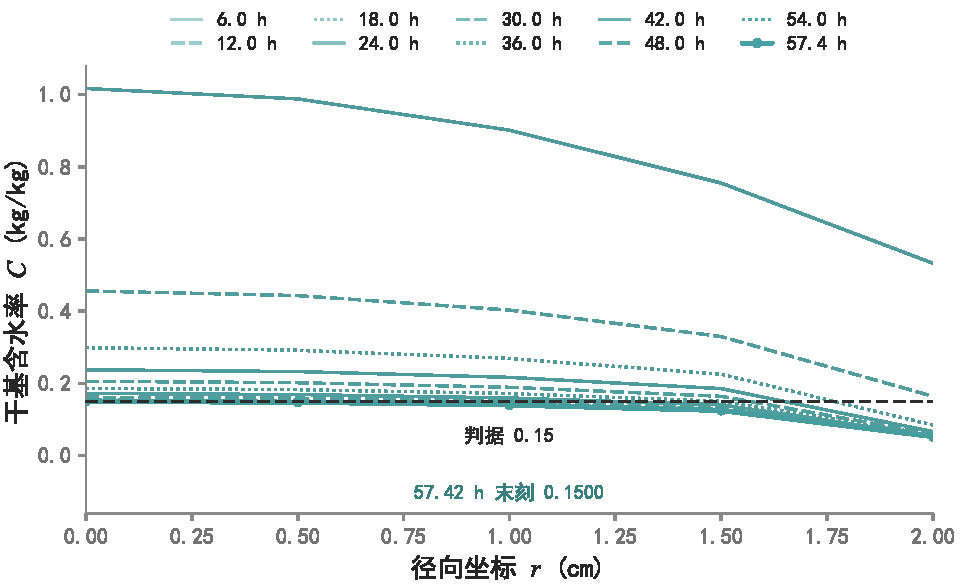
\includegraphics[width=0.9\textwidth,height=0.8\textheight,keepaspectratio]{../figures/fig_q3_profiles_6h.pdf}
  \caption{问题三每六小时径向剖面}
  \label{fig:q3_profiles_6h}
\end{figure}

每隔 $6$ h 取一条含水率剖面，可见所有剖面沿半径递减、形状逐条下移而不交叉
（图~\ref{fig:q3_profiles_6h}，图中标出 $0.15$ 阈值线）。数值上，
本算例全时空范围内的最大正向径向梯度为 $2.22\times10^{-15}$，
比单调性判据阈值 $10^{-9}$ 小六个量级，与双精度舍入同量级，
即未出现可分辨的正梯度。因此在本算例中空间最大值取于中心，
式~\eqref{eq:tdry_def}~的场判据与标量判据 $C(0,t)<0.15$ 给出相同的首达时刻，
可按式~\eqref{eq:tdry_interp}~在相邻 $60$ s 输出步之间线性插值定位。
这里的等价性来自实测单调性而非先验证明，故程序仍按全域最大值判定；
线性插值给出的是首达时刻的数值估计，其误差受输出步长 $60$ s 限制，
下文的时间步无关性检验给出该估计的稳定性。

图中还能读出另一件事：阈值线与各剖面的交点先出现在表面附近，
再逐条向中心移动，最后一条剖面在中心处刚好触到阈值。
这个几何图像正是“整根药材达标”与“中心达标”等价的直观来源。

\fi
\subsection{结果}

按 $N=160$、$\Delta t=1$ s 推进到第 $206\,760$ 步（即 $57.4333$ h）时判据首次满足，
在该步与前一输出步之间插值得

\begin{equation}
t_{\mathrm{dry}}=57.4247~\text{h}=2.3927~\text{d}.
\label{eq:tdry_q3}
\end{equation}

推进步数对应的时刻略迟于 $t_{\mathrm{dry}}$，二者相差不超过一个 $60$ s 输出步，
这是先跨过再回插的必然结果。
穿越确为首次：末输出步的 $\max_rC=0.149991$ 已低于阈值，
前一输出步为 $0.150008$ 仍高于阈值。全程离散守恒残差
$3.425\times10^{-10}$，说明式~\eqref{eq:global_balance}~的全局平衡
在数值解上逐步成立。

式~\eqref{eq:tdry_q3}~是一个条件式结论，其依赖关系在本节末尾定量给出：
$93.0\%$ 的时间轴由附件 1 末段平台的常数延拓提供边界条件，
该平台温度改变 $\pm0.5$ °C 时时长反向变化约 $1.6\%$。

\begin{figure}[!htbp]
  \centering
  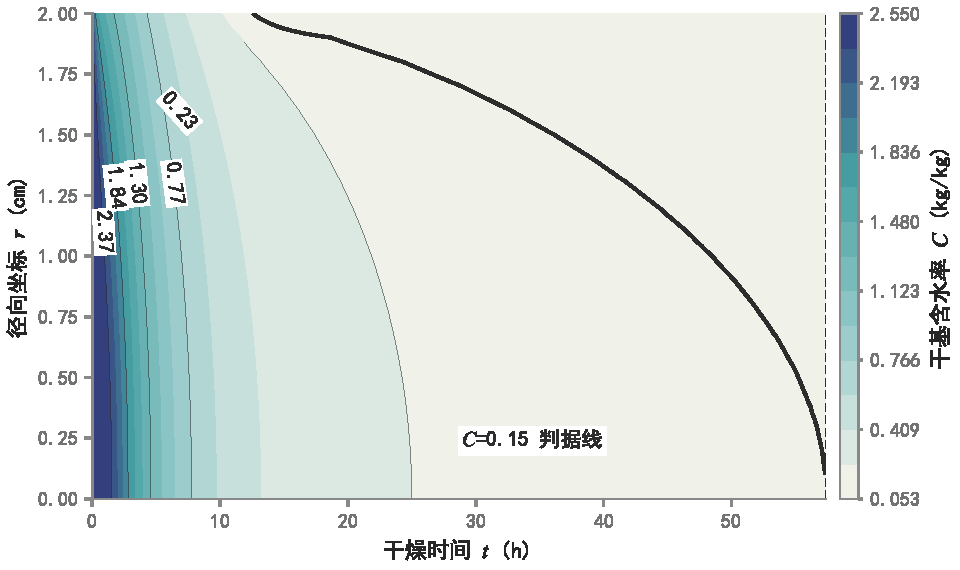
\includegraphics[width=0.9\textwidth,height=0.8\textheight,keepaspectratio]{../figures/fig_q3_field_C.pdf}
  \caption{问题三全程含水率场}
  \label{fig:q3_field_C}
\end{figure}

达标过程在时间上高度不均匀：$0.15$ 等值线在约 $12.6$ h 就抵达表面，
此后向中心推进的速度急剧变慢，最终在 $57.4247$ h 触及轴心——
这一时刻即式~\eqref{eq:tdry_q3}~的答案（图~\ref{fig:q3_field_C}~给出
$0$ 至 $57.42$ h 的全程含水率场并高亮该等值线）。等值线的减速形态与图~\ref{fig:q2_props_evolution}~中扩散系数
随含水率下降 $16.8$ 倍的强非线性直接对应：越接近达标，推进越慢。

式~\eqref{eq:tdry_q3}~落在题面给出的“一般持续 $2$ 至 $3$ 天”区间之内，
这是一条独立于本文模型的外部量级校核。

\begin{table}[H]
  \centering
  \caption{问题三烘干过程的水分浓度（kg/kg）}
  \label{tab:q3_C}
  \setlength{\tabcolsep}{4pt}
  \begin{tabular}{ccccccc}
  \toprule
  时间 (h) & $r=0$ cm & $r=0.5$ cm & $r=1.0$ cm & $r=1.5$ cm & $r=2.0$ cm & $\bar C$ \\
  \midrule
  6  & 1.0169 & 0.9881 & 0.9015 & 0.7550 & 0.5328 & 0.7817 \\
  12 & 0.4561 & 0.4431 & 0.4030 & 0.3297 & 0.1642 & 0.3367 \\
  18 & 0.2988 & 0.2915 & 0.2687 & 0.2253 & 0.0845 & 0.2270 \\
  24 & 0.2378 & 0.2327 & 0.2167 & 0.1855 & 0.0665 & 0.1858 \\
  30 & 0.2058 & 0.2018 & 0.1891 & 0.1640 & 0.0598 & 0.1639 \\
  36 & 0.1858 & 0.1825 & 0.1718 & 0.1503 & 0.0566 & 0.1499 \\
  42 & 0.1720 & 0.1691 & 0.1596 & 0.1406 & 0.0548 & 0.1401 \\
  48 & 0.1618 & 0.1591 & 0.1506 & 0.1334 & 0.0537 & 0.1328 \\
  54 & 0.1538 & 0.1514 & 0.1436 & 0.1276 & 0.0530 & 0.1270 \\
  烘干结束 57.4247 & 0.1500 & 0.1477 & 0.1402 & 0.1249 & 0.0526 & 0.1242 \\
  \bottomrule
  \end{tabular}
\end{table}

表~\ref{tab:q3_C}~的末行是烘干结束时刻，其余各处均已低于阈值，
中心值显示为 $0.1500$。这一显示值是四位小数舍入的结果，
未舍入值为 $0.149991$ kg/kg，已低于阈值；判据按未舍入值判定，
上一输出步的对应值为 $0.150008$ kg/kg，仍高于阈值，
两步之间正是插值定位的区间。表中同时给出干质量加权平均含水率一列，
便于读者核对前述均值判据与逐点判据的差别：第 $36$ h 行的 $\bar C=0.1499$
已达标而中心 $0.1858$ 未达标，两者的分歧一目了然。
同期温度在全部制表时刻、全部半径上均为 $50.0095$ °C，
四位小数下与平台温度不可分辨，故不单列温度表——
这再次印证问题二的判断：全程绝大部分时间里热已平衡，只有质在进行。
每隔 $60$ s、每隔 $0.1$ cm 的完整结果见 \verb|result3.xlsx|，
共 $3446$ 行 $\times$ $22$ 列，末行时刻已不早于 $t_{\mathrm{dry}}$。

\subsection{干燥动力学与烘房条件依赖}

\begin{figure}[!htbp]
  \centering
  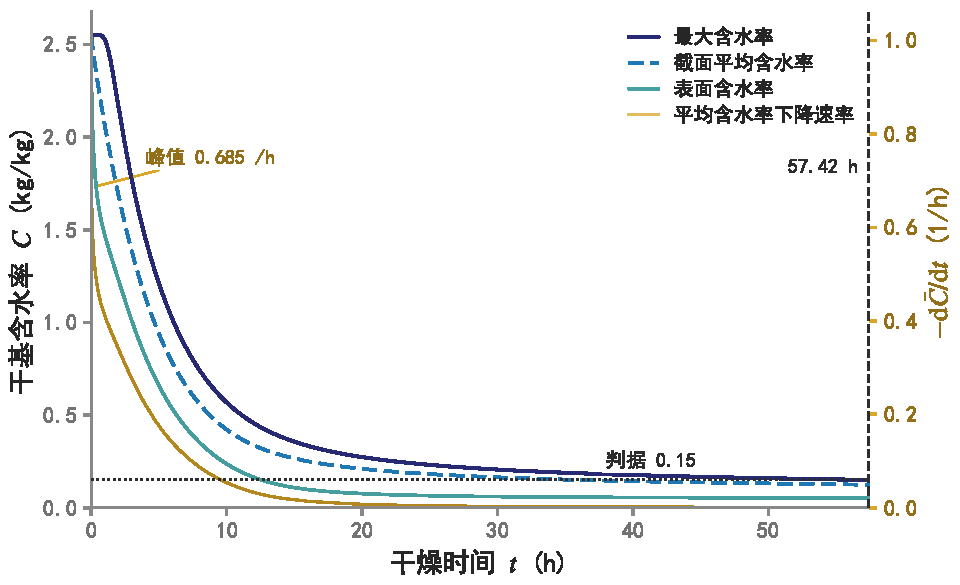
\includegraphics[width=0.9\textwidth,height=0.8\textheight,keepaspectratio]{../figures/fig_q3_drying_kinetics.pdf}
  \caption{问题三干燥动力学曲线}
  \label{fig:q3_drying_kinetics}
\end{figure}

本题工况下不存在恒速干燥段：三条含水率曲线全程不交叉，
干燥速率自始至终单调下降（图~\ref{fig:q3_drying_kinetics}~把中心、表面与
干质量加权平均含水率的时程与干燥速率画在双轴上）。这一“全程降速”特征与薄层热风干燥实验中
普遍观察到的形态一致\upcite{chigbo2024thinlayer,rodriguez2014thyme}，
说明本题工况下干燥速率始终由内部扩散控制，而非由表面汽化控制；表面含水率到 $18$ h 已降至 $0.0845$ kg/kg，
此后缓慢趋近空气含湿量 $0.05$ 的量级，成为内部水分的出口而不是限制环节。图中中心与平均两条曲线的间距
就是均值判据偏短的来源。

由于式~\eqref{eq:tdry_q3}~的时间跨度远超附件 1 的覆盖范围，
必须把该结果的条件性一并说清。附件 1 实测只覆盖前 $4$ h，
占总时长的 $7.0\%$；其余 $93.0\%$ 的时间轴由平台均值常数延拓段支配。
第~\ref{sec:validation}~节的单因子扰动给出该依赖的定量边界：
平台温度改变 $\pm0.5$ °C 时烘干时长反向变化约 $1.6\%$，折合约 $0.9$ h。
因此式~\eqref{eq:tdry_q3}~应理解为“在恒温平台取附件 1 末段均值前提下”
的烘干时长。作为鲁棒性对照，若改用末点值 $50.1650$ °C 而非均值
$50.0095$ °C 作延拓，两者相差 $0.1555$ °C，已被上述 $\pm0.5$ °C 的
扰动幅度覆盖。

\subsection{网格与时间步无关性}

$N=160$ 已满足相邻相对差 $5\times10^{-4}$ 判据；从 $\Delta t=4$ s 收至 $0.5$ s，$t_{\mathrm{dry}}$ 仅改变约 $3\times10^{-3}$ h。完整收敛图表见附录 C。
\iffalse

阈值首达时刻是一个由整条时程累积而来的量，比场值更容易受离散误差影响，
因此需要专门核查。

\begin{figure}[!htbp]
  \centering
  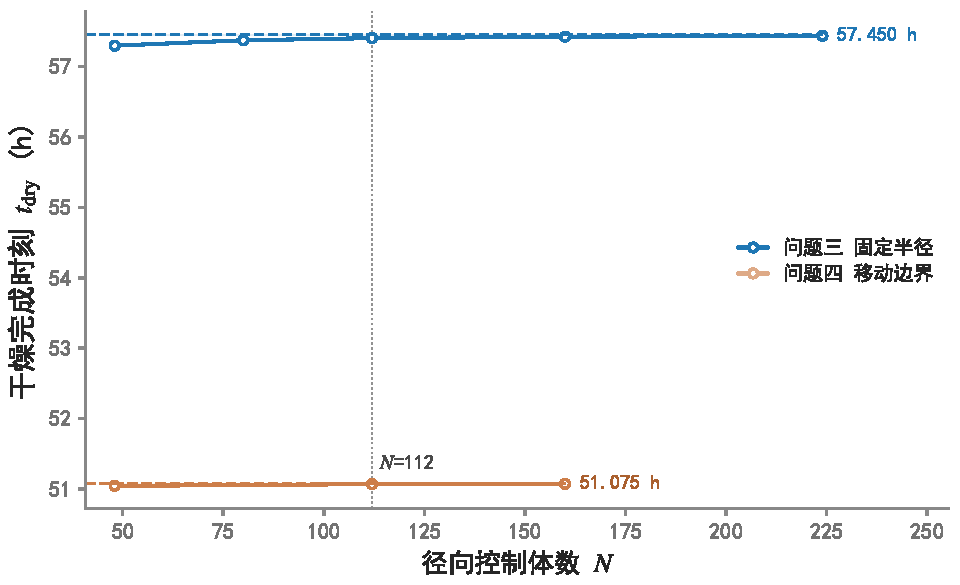
\includegraphics[width=0.9\textwidth,height=0.8\textheight,keepaspectratio]{../figures/fig_grid_convergence.pdf}
  \caption{网格收敛性检验}
  \label{fig:grid_convergence}
\end{figure}

两问的 $t_{\mathrm{dry}}$ 都随网格加密单调趋于稳定值，
相邻相对差在生产网格处已进入 $5\times10^{-4}$ 判据以内
（图~\ref{fig:grid_convergence}~给出两条收敛轨迹并标出该判据，
问题三一侧的具体数值列于表~\ref{tab:grid}）。

\begin{table}[H]
  \centering
  \caption{问题三网格收敛性}
  \label{tab:grid}
  \begin{tabular}{rrr}
  \toprule
  径向控制体数 $N$ & $t_{\mathrm{dry}}$ (h) & 相对前一档差 (\%) \\
  \midrule
  48  & 57.2968 & --     \\
  80  & 57.3738 & 0.1343 \\
  112 & 57.4040 & 0.0527 \\
  160 & 57.4247 & 0.0360 \\
  224 & 57.4370 & 0.0214 \\
  \bottomrule
  \end{tabular}
\end{table}

表~\ref{tab:grid}~的相对差列单调下降，末两档均已优于 $5\times10^{-4}$ 判据。
细化网格使 $t_{\mathrm{dry}}$ 单调略微变长，说明粗网格会低估烘干时长，
其机理是控制体过少时表面附近的陡梯度被抹平、表面通量被高估。
补充网格集 $N\in\{40,60,80,120,160\}$ 给出的相对差由 $1.390\times10^{-3}$
降到 $2.770\times10^{-4}$，同样单调，排除了收敛轨迹依赖于特定网格序列的可能。

\begin{table}[H]
  \centering
  \caption{问题三时间步收敛性}
  \label{tab:dt}
  \begin{tabular}{rr}
  \toprule
  时间步 $\Delta t$ (s) & $t_{\mathrm{dry}}$ (h) \\
  \midrule
  4.0 & 57.4067 \\
  2.0 & 57.4049 \\
  1.0 & 57.4040 \\
  0.5 & 57.4036 \\
  \bottomrule
  \end{tabular}
\end{table}

表~\ref{tab:dt}~在 $N=112$ 下固定空间网格单独考察时间步，
八倍的步长变化只改变 $3.0\times10^{-3}$ h，比表~\ref{tab:grid}~中同一档位
$N=112$ 的相邻网格差 $3.0\times10^{-2}$ h 小一个数量级。两表合起来说明
空间离散是误差主项、时间离散不是。生产配置 $N=160$、$\Delta t=1$ s 的
残余离散误差可由最密一档估计：$N=224$ 给出 $57.4370$ h，
与生产值相差 $0.0123$ h（约 $44$ s），相对量 $2.1\times10^{-4}$。
因此式~\eqref{eq:tdry_q3}~在小时量级上是稳定的，
但其末位小数不应按有效数字解读——本文保留四位小数只为便于复核，
可信区间由上述 $0.0123$ h 给出。
这也解释了后向 Euler 格式一阶时间精度在此并不构成限制：
烘干过程的时间尺度是数十小时，$1$ s 的步长相对之下极小。
\fi
